\documentclass[]{report}
\usepackage{graphicx}

% Title Page
\title{A Report into the Relationship between Tax, GDP and Regulatory Environment}
\author{Your name goes here}


\begin{document}
\maketitle

\begin{abstract}
A Report compiled for the Alliance of Wealthy People who Dislike Tax, investigating the relationship between rates of taxation (measured as a percentage of GDP), regulatory environment (measured through the World Bank's Ease of Doing Business), and GDP per capita (measured in current US dollars). Data are for European and Central Asian countries for the year 2019.
\end{abstract}

\section{Findings}
A multivariate regression of the variables resulted in the following findings:

% Table created by stargazer v.5.2.3 by Marek Hlavac, Social Policy Institute. E-mail: marek.hlavac at gmail.com
% Date and time: Thu, Jan 25, 2024 - 13:17:38
\begin{table}[!htbp] \centering 
	\caption{} 
	\label{} 
	\begin{tabular}{@{\extracolsep{5pt}}lc} 
		\\[-1.8ex]\hline 
		\hline \\[-1.8ex] 
		& \multicolumn{1}{c}{\textit{Dependent variable:}} \\ 
		\cline{2-2} 
		\\[-1.8ex] & )` \\ 
		\hline \\[-1.8ex] 
		`Tax revenue (\% of GDP)` & 1,478.218$^{**}$ \\ 
		& (729.778) \\ 
		& \\ 
		`Ease of doing business rank (1=most business-friendly regulations)` & $-$216.435 \\ 
		& (161.963) \\ 
		& \\ 
		Constant & 8,572.687 \\ 
		& (17,117.090) \\ 
		& \\ 
		\hline \\[-1.8ex] 
		Observations & 46 \\ 
		R$^{2}$ & 0.137 \\ 
		Adjusted R$^{2}$ & 0.097 \\ 
		Residual Std. Error & 24,727.080 (df = 43) \\ 
		F Statistic & 3.416$^{**}$ (df = 2; 43) \\ 
		\hline 
		\hline \\[-1.8ex] 
		\textit{Note:}  & \multicolumn{1}{r}{$^{*}$p$<$0.1; $^{**}$p$<$0.05; $^{***}$p$<$0.01} \\ 
	\end{tabular} 
\end{table} 

The relationship can be visualised in a scatter plot.
%edit this code with the name of the pdf of your plot. This must be in the same directory as this .tex file
\begin{figure}[b!]\centering
	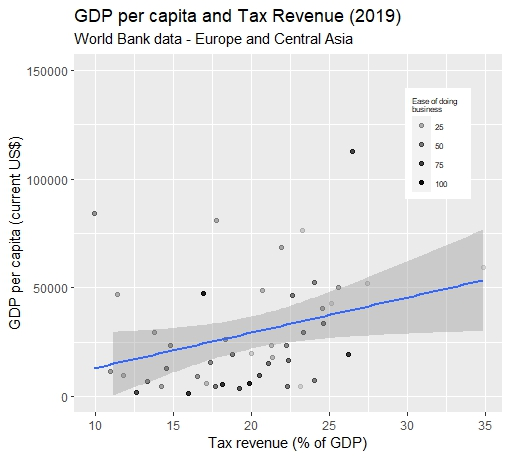
\includegraphics[width=\textwidth]{Rplot01.jpeg}\\
\end{figure}

\end{document}          
